\documentclass[peerreview]{ieeesyscoin}
\usepackage{cite}
\usepackage{amsmath,amssymb,amsfonts}
\usepackage{algorithmic}
\usepackage{enumitem}
\usepackage{caption}
\usepackage{xcolor}
\usepackage{graphicx}
\usepackage{textcomp}
\usepackage{multirow}
\usepackage[switch]{lineno}
\def\BibTeX{{\rm B\kern-.05em{\sc i\kern-.025em b}\kern-.08em
    T\kern-.1667em\lower.7ex\hbox{E}\kern-.125emX}}
\begin{document}
\linenumbers
\history{}

\title{\centering Syscoin 4.0: A Peer-to-Peer Electronic Cash System Built For Business Applications}
\author{\centering  \uppercase{Jagdeep Sidhu, MSc}\authorrefmark{1}, 
and \uppercase{Ian C. Moore, PhD\authorrefmark{2}}}

\address[1]{\centering Syscoin Core Developer, Blockchain Foundry Inc.(e-mail: jsidhu@blockchainfoundry.co)}
\address[2]{\centering  (e-mail: ic3moore@gmail.com)}
\tfootnote{}

\markboth
{Sidhu \headeretal: Syscoin 4.0: A Peer-to-Peer Electronic Cash System Built For Business Applications}
{Sidhu \headeretal: Syscoin 4.0: A Peer-to-Peer Electronic Cash System Built For Business Applications}

\corresp{}

\begin{abstract}
Syscoin 4.0 introduces a novel implementation of a decentralized identityz masternodes providing bonded validators for a PoW/PoS hybrid consensus model (DAG) / zero knowledge proofs and instant pseudo-interactive zero-confirmation cryptocurrency transactions with double-spend protection.
\end{abstract}

\begin{keywords}
Network EVM, DAG, Decentralized Identity, Zero Knowledge Proofs
\end{keywords}

\titlepgskip=-15pt

\maketitle

\section{Introduction}
\label{sec:introduction}

Syscoin 4.0 builds upon Syscoin 3.0 with additional implementation of an Ethereum Bridge, Offers/Escrow, Lightening Networks, and Decentralized Identity. As previously featured, anything pertaining to the market place (eg, digital sales, auctions, marketplace modification, etc.) has been deprecated. The full release will included the Syscoin Network-Enhanced Virtual Machine (NEVM) which will utilize the Ethereum Virtual Machine (EVM) together with a Zero Knowledge Proof (ZKP) system to build scalable applications and the introduction of a decentralized cost model around Ethereum Gas fees (Table \ref{table:ugrades}).

High Gas fees and low transaction throughput are some of the key issues that are hindering ERC-20 projects from running at scale. However, Ethereum 2.0 is currently under development to address these issues, where its final release is anticipated to be completed several years from now. Instead of building a competing smart contract system, we have decided to work with the EVM protocol, and to provide a faster and cost effective alternative to what Ethereum 2.0 is proposing. The roadmap for Syscoin 4.0 proposes a four-layer tech stack to address this using: (a) Syscoin as the base layer to provide security; (b) EVM for programmability; (c) ZKP for scalability; and (d) applications to provide decentralized usability for the next phase of the Internet's evolution, known as Web 3.0. 

In Section \ref{sec:protocol} we address the protocol attributes, which include ZDAG, order-of-events, point-of-sale applications, assets, non-fungible tokens, lightning networks, offers/escrow, and masternodes. In Section \ref{section:roadmap} we lay out the roadmap for Syscoin 4.0, which includes scalability, design proposal, evidence, and applications. In Section \ref{section:specs} we outline the protocol specifications, followed by the conclusion in Section \ref{section:conclusion}.

\begin{table}[h!]
\caption{Syscoin 4.0 Upgrades and Modifications}
\label{table:ugrades}
\setlength{\tabcolsep}{3pt}
\begin{tabular}{|p{135pt}|p{75pt}|}
\hline
Syscoin Feature & 
Update (from 3.0) \\

\hline
Nakamoto ZDAG (ie, Z-Dag) & no change \\
Assets & modified \\

Offers and decentralized marketplace &   \\
~~~~~ Digital Sales &  deprecated \\
~~~~~ Auctions &  deprecated \\
~~~~~ Reselling w/ whitelists &  modified \\
~~~~~ Feedback and rating &  deprecated \\
~~~~~ Multiple payment options &  deprecated \\
~~~~~ Shipping notification system &  deprecated \\
~~~~~ Marketplace moderation &  deprecated \\

Data Anchoring &  deprecated \\
Instant Encrypted Messages &  re-purposed \\
Blockchain pruning &  deprecated \\
Certificates (see Identity) &  modified \\
Decentralized Identity &  new feature \\
~~~~~ Certificates &  modified \\
Lightning networks &  new feature \\
Offers / Escrow &  new feature\\
Roadmap to Web 3.0 & \\
~~~~~ Network EVM (NEVM) &  proposed  \\
~~~~~ Zero Knowledge Proofs &  proposed \\
~~~~~ NEVM Applications &  proposed \\

\hline
\multicolumn{2}{p{251pt}}{depreciated  $\rightarrow$ removed from 4.0; modified  $\rightarrow$ repurposed from 3.0; new feature  $\rightarrow$ upgrade from 3.0; no update $\rightarrow$ carry-over from 3.0}\\

\end{tabular}
\label{tab1}
\end{table}


\section{Protocol Characteristics}
\label{sec:protocol}

\subsection{Z-DAG}
Z-DAG (Zero-Confirmation Directed
Acyclic Graph) is an instant settlement protocol functioning
across all Syscoin services. Syscoin services consist of
Alias Identities, Certificates, Escrow, Offers and Assets.
Each service is controlled via an Alias, in which ownership
is proven through a private key that matches each
unique address. Z-DAG organizes transactions based on
dependencies to build the state in a deterministic fashion.
This helps protect against double spends where an Asset is
transferred falsely by creating multiple transactions through
multiple nodes within a short time.

Figure 1 shows the difference between a regular
blockchain and Syscoin’s Z-DAG implementation. Syscoin
now has two consensus layers: In the first layer, a ZDAG graph of transactions are represented in the mempool
without a block, providing settlement in real-time. The secondary layer provides confirmation and conflict resolution
preventing double-spend events through existing Proof of
Work consensus.

Verifying client nodes creates a graph of transactions
by looking at the sender/receiver list of Asset transfers. A
circuit detection algorithm is applied (read below Hawick
cycle detection) and used to remove cycles from within the
graph to create a DAG (Directed Acyclic Graph). Once the
DAG is created it is topologically sorted with an Asset
transfer consensus code being processed in sequence, to
form a deterministic state among the entire network in
consensus.

Z-DAG can be applied to state changes (similar to
UTXO updates to Bitcoin). If any discrepancy occurs, Proofof-Work (PoW) will override and replay the correct order
of events according to the miner; this is ensured by saving
the previous state on every block and rolling back to the
previous state prior to every block.

A User Interface layer will notify the user of conflicts
in real-time, making the transaction occur between 3-5
seconds (statistically the amount of time needed to ensure
that network takes to notice that 2 double spend transactions
are conflicting with each other). This is possible through
Syscoin’s Masternode layer. Every Masternode is connected
to 25 or more peers providing high-throughput relay across
the network, averaging one or more network hops to transmit
from the sender to the receiver nodes.

The partition tolerance of the protocol is the PoW block
timing which is set to 60 seconds on Syscoin 3. Every block,
a new DAG is constructed from the transactions within that
block. Unlike other implementations that have no PoW to
fall back on, there is no case where the DAG tends toward an
incorrect state over time.To accurately detect double-spends,
other implementations such as Phantom[SZ] or Spectre[Zoh]
must use an algorithm to replace the longest chain rule to
derive the order of events and attacker sequences in a graph.
These implementations end up in a more complex gametheoretical situation that has not mathematically been proven
to be accurate in all cases. Syscoin relies on the thoroughly
tested Nakamoto consensus model to arrive at a consensus
over time rather than simply relying on a DAG.

\subsection{Order-of-events preservation and Conflict Resolution}
Mauris ipsum. Nulla metus metus, ullamcorper vel, tincidunt sed, euismod in, nibh. Quisque volutpat condimentum velit. Class aptent taciti sociosqu ad litora torquent per conubia nostra, per inceptos himenaeos. Nam nec ante. Sed lacinia, urna non tincidunt mattis, tortor neque adipiscing diam, a cursus ipsum ante quis turpis. Nulla facilisi. Ut fringilla. Suspendisse potenti. Nunc feugiat mi a tellus consequat imperdiet. Vestibulum sapien. Proin quam. Etiam ultrices. Suspendisse in justo eu magna luctus suscipit. 


\subsection{CAP Theorem}
The CAP theorem[Bre] states that it is impossible for
a distributed data store to simultaneously provide more
than two out of the following three guarantees: consistency,
availability or partition tolerance. Bitcoin tries to provide a
guarantee that transactions are settled, but mathematically
it is not able to do so. Z-DAG trades some consistency for
some availability. Since it is unlikely that a double-spend or
re-organization will change the state of someone’s balance,
we do not wait for settlement finality by waiting for blocks
to confirm. This drastically increases the usability in pointof-sale applications.

The allowance of instant settlements and increased availability requires paying additional attention to users simply
trying to double-spend or send transactions too quickly,
which may cause the miner view to change from the general
network view. The DAG will order the dependency graph
of transactions and process in sequence, allowing for better
availability when it comes to instant state changes. The
same CAP constraints as Proof-of-Work will provide a more
responsive money transfer mechanism that may be used as
a transaction processor instead of simply a settlement layer.

\subsection{Point-of-sale applications}
The combination of using Assets with Z-DAG will allow for point-of-sale applications, providing service in real-time exchange for cryptocurrency Asset tokens.

\subsection{Assets}
Sed lectus. Integer euismod lacus luctus magna. Quisque cursus, metus vitae pharetra auctor, sem massa mattis sem, at interdum magna augue eget diam. Vestibulum ante ipsum primis in faucibus orci luctus et ultrices posuere cubilia Curae; Morbi lacinia molestie dui. Praesent blandit dolor. Sed non quam. In vel mi sit amet augue congue elementum. Morbi in ipsum sit amet pede facilisis laoreet. Donec lacus nunc, viverra nec, blandit vel, egestas et, augue. Vestibulum tincidunt malesuada tellus. Ut ultrices ultrices enim. Curabitur sit amet mauris. 

\subsection{Non-Fungible Tokens}

Sed lectus. Integer euismod lacus luctus magna. Quisque cursus, metus vitae pharetra auctor, sem massa mattis sem, at interdum magna augue eget diam. Vestibulum ante ipsum primis in faucibus orci luctus et ultrices posuere cubilia Curae; Morbi lacinia molestie dui. Praesent blandit dolor. Sed non quam. In vel mi sit amet augue congue elementum. Morbi in ipsum sit amet pede facilisis laoreet. Donec lacus nunc, viverra nec, blandit vel, egestas et, augue. Vestibulum tincidunt malesuada tellus. Ut ultrices ultrices enim. Curabitur sit amet mauris. 

\subsection{Decentralized Identity}
Sed lectus. Integer euismod lacus luctus magna. Quisque cursus, metus vitae pharetra auctor, sem massa mattis sem, at interdum magna augue eget diam. Vestibulum ante ipsum primis in faucibus orci luctus et ultrices posuere cubilia Curae; Morbi lacinia molestie dui. Praesent blandit dolor. Sed non quam. In vel mi sit amet augue congue elementum. Morbi in ipsum sit amet pede facilisis laoreet. Donec lacus nunc, viverra nec, blandit vel, egestas et, augue. Vestibulum tincidunt malesuada tellus. Ut ultrices ultrices enim. Curabitur sit amet mauris. 

\subsubsection{Selfish mining}

Integer lacinia sollicitudin massa. Cras metus. Sed aliquet risus a tortor. Integer id quam. Morbi mi. Quisque nisl felis, venenatis tristique, dignissim in, ultrices sit amet, augue. Proin sodales libero eget ante.

\subsubsection{Chain locks}

With a subset of nodes offering sybil resistance through the requirement of bonding 100,000 SYS to become active, plus the upcoming deterministic masternode feature in Syscoin 4.2, we have enabled Chain Locks which attempts to solve a long-standing security problem in Bitcoin \cite{Eya18}, where Dashcore was the first project to implement this idea \cite{Blo18} which the industry has since widely accepted as a viable solution \cite{Val19}. Our implementation is an optimized version of this, in that we do not implement Instant Send or Private Send transactions and thus Syscoin’s Chain Lock implementation is much more simpler. Because of merged-mining functionality with Bitcoin, we believe our chain coupled with Chain Locks becomes the most secure via solving Bitcoin’s most vulnerable attack vector, selfish mining. 

These Chain Locks are made part of Long-Living Quorums (LLMQ) which leverage aggregatable Boneh–Lynn–Shacham (BLS) signatures that have the property of being able to combine multiple signers in a Distributed Key Generation (DKG) event to sign on decisions. In this setup, a signature can be signed on a group of parties under threshold constraints without any one of those parties holding the private key associated with that signature. In our case, the signed messages would be a ChainLock Signature (CLSIG) which represent claims on what the block hashes represent of the canonical chain \cite{Blo18}. This model suggests a very efficient   threshold signature design was needed to be able to quickly come to consensus across the Masternode layer to decide on chain tips and lock chains preventing selfish mining attacks. See \cite{Bon18} to understand the qualities of BLS signatures in the context of multi-sig use cases.

Ethereum 2.0 design centers around the use of BLS signatures through adding precompile opcodes in the Ethereum Virtual Machine (EVM) for the BLS12-381 curve \cite{Dra18} which Syscoin has adopted. This curve was first introduced in 2017 by Bowe \cite{Bow17}  to the ZCash protocol. Masternodes on Syscoin use this curve and have a BLS key that is associated with each validator. There is the performance comparison to ECDSA (Secp256k1) \cite{Blo18} that shows its usefulness in contrast to what Bitcoin and Syscoin natively use for signature verification.

\subsubsection{Reselling and Whitelists}

Curabitur sodales ligula in libero. Sed dignissim lacinia nunc. Curabitur tortor. Pellentesque nibh. Aenean quam. In scelerisque sem at dolor. Maecenas mattis. Sed convallis tristique sem. Proin ut ligula vel nunc egestas porttitor. Morbi lectus risus, iaculis vel, suscipit quis, luctus non, massa. Fusce ac turpis quis ligula lacinia aliquet. Mauris ipsum. 

\subsection{Lightning Networks}
Proin ut ligula vel nunc egestas porttitor. Morbi lectus risus, iaculis vel, suscipit quis, luctus non, massa. Fusce ac turpis quis ligula lacinia aliquet. Mauris ipsum. Nulla metus metus, ullamcorper vel, tincidunt sed, euismod in, nibh. Quisque volutpat condimentum velit. Class aptent taciti sociosqu ad litora torquent per conubia nostra, per inceptos himenaeos. Nam nec ante. Sed lacinia, urna non tincidunt mattis, tortor neque adipiscing diam, a cursus ipsum ante quis turpis. Nulla facilisi. Ut fringilla. Suspendisse potenti. Nunc feugiat mi a tellus consequat imperdiet. 

\subsection{Offers / Escrow}
Vestibulum sapien. Proin quam. Etiam ultrices. Suspendisse in justo eu magna luctus suscipit. Sed lectus. Integer euismod lacus luctus magna. Quisque cursus, metus vitae pharetra auctor, sem massa mattis sem, at interdum magna augue eget diam. Vestibulum ante ipsum primis in faucibus orci luctus et ultrices posuere cubilia Curae; Morbi lacinia molestie dui. Praesent blandit dolor. Sed non quam. In vel mi sit amet augue congue elementum. Morbi in ipsum sit amet pede facilisis laoreet. Donec lacus nunc, viverra nec, blandit vel, egestas et, augue. Vestibulum tincidunt malesuada tellus. 

\subsection{Masternodes}

With 2400+ masternodes running fullnodes, Z-DAG becomes much more dependable, as does the propagation of blocks and potential forks. The masternodes are bonded through a loss-less strategy of putting 100000 Syscoin in an output and running full nodes in exchange for block rewards. A seniority model incentivizes the masternodes to share long-term growth by paying them more for the longer period of service. Half of the transaction fees are also shared between the PoW miners and masternodes to ensure long term alignment once subsidy becomes negligible. The coins are not locked at any point, and there is no slashing condition if masternodes decide to move their coins, the rewards to those masternodes simply stop. Sharing Bitcoin’s compact block design, it consumes very little bandwidth to propagate blocks assuming the memory pool of all these nodes is roughly synchronized \cite{BitCore}. The traffic on the network primarily consists of propagating the missing transactions to validate these blocks. Having a baseline for a large number of full-nodes that are paid to be running allows us to create a very secure environment for users. It proposes higher costs to would-be attackers who either have to attempt a 51\% attack of Syscoin (effectively also trying to attack the Bitcoin network), or try to game the mesh network by propagating bad information which is made more difficult by incentivized full-nodes. The health of a decentralized network consists of the following; (a) the mining component or consensus to produce blocks, and (b) the network topology to disseminate information in a timely manner in conditions where adversaries might be lurking. Other attacks related to race conditions in networking or consensus code are mostly negligible as Syscoin follows a rigorous and thorough continuous development process. This includes deterministic builds, Fuzz tests, ASAN/MSAN/TSAN, functional/unit tests, multiple clients and adequate code coverage. Syscoin and Bitcoin protocol code bases are merged daily such that the build/signing/test processes are all identical, allowing us to leverage the massive developer base of Bitcoin. The quality of code is reflective of taking worst case situations into account. The most critical engineers and IT specialists need confidence that value is secure should they decide to move their business to that infrastructure. It’s true that there are numerous new ideas, new consensus protocols and mechanisms for achieving synchronization among users in a system through light/full node implementations. However, in our experience in the blockchain industry over the last eight years, we understand that it takes years, sometimes generations to bring those functionalities to production level quality useful for commercial applications. 

\section{Roadmap to Web 3.0}
\label{section:roadmap}

Bitcoin was the first to attempt to offer a practical outcome in the General's Dilemma using Crypto Economic rationale and incentives. Ethereum was the first to abstract the concept of turing completeness within similar frameworks assumed by Bitcoin. What Syscoin presents is a combination of both Bitcoin and Ethereum with intuitions built on top to achieve a more efficient financial computing platform which leverages coordination to achieve consensus using Crypto Economic rationale and incentives. We propose a four-layer tech stack using Syscoin as the base (host) layer, which provides an efficient (ie, low gas cost per transaction) platform. Some of the main advantages include building scalable decentralized applications, the introduction of a decentralized cost model around Ethereum Gas fees. This new model proposes state-less parallelized execution and verification models while taking advantage of the security offered by the Bitcoin protocol. We may also refer to this as Web 3.0.

\subsection{Scalability and Security}

Scalability in blockchain environments is typically measured by total Transactions per Second (TPS). This suggests full trustlessness, decentralization and liveness properties as evidenced by something like Bitcoin. If trade-offs are made to achieve higher scale, it means another property is affected. A full node is one that creates blocks and/or fully validates every block of transactions. For the purpose of this discussion, we will refrain on expounding on designs where light-clients are used to give semblance of higher throughput, etc. However, if two nodes are running the same hardware and doing the same work, the one that provides more TPS performance than the other is considered more scalable. This is not to be confused with throughput which is the measure of output that can be increased by simply adding more hardware resources. Hence, more throughput does not mean more scalable. Some blockchains require the producers of blocks to run on higher specifications, offering higher throughput but not necessarily more scale. However, there are projects which employ parallel processing to try to achieve higher scale whilst also enforcing more capable hardware to provide a more efficient overall system [33]. As a logical experiment, the throughput of a system divided by the scalability of the system is what we define as efficiency. In the following sections, we will outline our proposal for improved efficiency.

\subsubsection{Efficiency}

The holy grail of blockchain design resides in the ability to have a ledger that can claim to be sublinear while retaining consistency, fault tolerance, and full availability (ie, CAP Theorem). This concedes  there are roughly constant costs for an arbitrary amount of computation performed and being secured by that ledger. This has always been thought of as impossible and it mostly is unless acceptable trade-offs appear in application designs if  they are easy to understand and work around. Most experts make the assumption that an O(1) ledger is simply impossible and thus design blockchains and force applications to work in particular ways as a result. We will remove such assumptions and let business processes dictate how they work by giving the ability to achieve O(logk n) for some constant k (ie, polylogarithmic) efficiency with trade-offs. A polylogarithmic design would give the ability for almost infinite scaling over time for all intents and purposes. The only bottlenecks proposed are fast information that can be propagated across the network. This in turn would improve over time as telecom infrastructure naturally evolves and increases in both capability and affordability.

Put in context, even Lightning Networks for transactional counts qualifies as a form of sublinear scaling on a transactional basis but not per user, as users must necessarily enter the main chain first before entering a payment channel. It requires the state of the blockchain to include the users joining the system. This state (the UTXO balances) is the primary  factor of efficiency degradation in Bitcoin. Users need to first start on the main chain and then move into the payment channel system to receive money, meaning that scale is at best O(N) where N is the number of users. There are some solutions to this problem of state storage on Bitcoin by reducing it via an alternative accumulator strategy to the cost of increased bandwidth \cite{Dry19}. This approach would make the chain state-less,  however the validation costs would remain linear to the number of transactions being done. When combined with payment channels, only the costs to get in/out are factored into the validation. This offers an interesting design for payments themselves while providing for on-chain availability. We consider this as a satisfactory path for futuristic scalable payments. Hence, it is not possible to employ that strategy with general computations. With this design, we are still left with the issue on how to do general computations at higher efficiency.

What we present is the ability to have a polylogarithmic chain at the cost of availability for both payments and general computations where business processes dictate availability policies, and users fully understand these limitations when using such systems. Users will ensure availability for themselves and others at their discretion.  This will be expanded upon in the following sections.

\subsubsection{State Liveness and State Safety}

While many compelling arguments can be made migrating to a state-less design \cite{Hot19}, it is not possible to achieve sublinear efficiency without sacrificing some other desired component that we outlined above. To achieve polylogarithmic efficiency, it’s necessary to have a mix of state and stateless nodes working together in harmony on a shared ledger \cite{Hot19}. This should be accomplished so that business processes can dictate direction, and users can choose to pay a little more for security either by using a stateful yet very scalable ledgering mechanism or by paying to ensure their own data availability amortized over the life of that user on such systems. Presenting the ability for users to make these choices allows us to separate the consensus of such systems and reduce overall complexity. However, in whatever solution we adopt , we need to ensure that the final implementation allows for both the liveness and safety of that state, which are defined as follows:

\begin{itemize}
\item \textbf{State Liveness}: Transferring coins in a timely manner
\item \textbf{State Safety}:  Private custody
\end{itemize}

It is important to adhere to these concepts; if one cannot move one’s coins, then it is as useful as if one burned their coins. Hence, if we had third party custody in place, this would give rise to custodial solutions. The loss of decentralized and trustless aspects of the solution is not desired. 

The options as described would allow users to decide their state liveliness at their own discretion, while state safety is a required constraint throughout any system design we provide. The doorway to possibilities of sublinear design is opened by giving users the ability to decide.


\subsubsection{Avoiding Re-execution of Transactions}

In order to scale arbitrarily, independent of the number of transactions - a desired property of increasing throughput - one requires a mechanism to avoid re-executing transactions \cite{Bow18}. Ideally, it would be able to batch these transactions together for a two-fold scaling proposition. There are a few mechanisms in literature that attempted to solve re-execution:
(a) TrueBit; (b) Plasma; and (c) Arbitrum avoided re-execution. Unfortunately, they require challenge response systems to ensure security, which leads to intricate attack vectors of unbounded risk/reward scenarios. 

Multi-Party Computation (MPC) is a mechanism to have parties act under a threshold to decide on actions such as computational integrity of a smart contract. MPC is used in Syscoin for BLS threshold signatures for Chain Locks and Proof-of-Service in quorums of validators deterministically chosen using Fiat-Shamir heuristics on recent block hashes. The problem with this approach is that validators may become corrupt, hence they need to be wrapped in a consensus system along with DKG and random deterministic selection. This was an interesting topic of discovery for the Syscoin team in the preliminary stages as a way to potentially scale smart contract execution.  It was ultimately discarded due to the incentive for risk/reward scenarios to favour attacks as the value of the transactions increases.

Hardware enclaves (eg, Intel SGX through remote attestation) were also of particular interest to the Syscoin team as a way to offload execution and avoid re-execution costs. However, there are a myriad of attack vectors and censorship concerns on the Intel platform . We also should note that the Antarctica model was interesting but required a firmware update from Intel to support such a feature which raises concerns over censorship long term \cite{Nil20}.

The theme amongst all of these approaches is that although re-execution is avoided the communication complexity is largely still linear with the number of transactions on the main chain. The security and trust models are also different from that of the layer 1 assumptions which was not desired.

Lacking solvent solutions to avoid re-execution and enable sublinear overall complexity, we were led - in the development of Syscoin 4.0 - to build a trust-minimized two-way bridge between Syscoin and the Ethereum mainchain, offloading the concerns around smart contracts to Ethereum. With the advent of such promising technology as ZKP and the optimizations happening around them [18, 19], we have re-considered the possibilities and believe this will have an integral role in the development of Web 3.0. This mathematical breakthrough led us to re-test our assumptions and options related to our desired design.

ZKP allows us the desired superlinear scaling trait we had been looking to achieve but they also offer other benefits; namely privacy is very easy to introduce and will not add detectable costs and complexities to verification on the mainchain. With users controlling their own data, the mainchain and systems may be designed such that only balance adjustments are recorded, not transaction sets (we will explain the case with full data availability below). In this scenario there is no advantage for a miner to gain to be able to collude with users to launch attacks on systems such as Decentralize Finance (DeFi) pools and provenance of transactions. The flexibility has to be present for application developers that need experiences consistent with those we have today with Bitcoin/Syscoin/Ethereum. This would enable the privacy use-cases without requiring extra work, knowledge or costs.


\subsubsection{Validity Proof Systems Overtop Proof-of-Work Systems}

Prior to the use of Proof Systems, the only option for “Validity Proofs” in a permissionless system involved naive replay, and as such greatly limited scalability Essentially, this replay is what is still done today in Layer-1 blockchain (L1) solutions, with the known penalty to scalability. Proof Systems offer a very appealing trait known as succinctness: in order to validate a state transition, one needs to only verify a proof, and this is done at a cost that is effectively independent of the size of the state transition (ie, polylogarithmic in the size of the state transition).

For maximal financial security, the amount of value being stored should depend on the amount of security provided on the settlement side of the ledger. Proof-of-Work offers the highest amount of security guarantees. Our next generation financial systems begin with optimal ledgering security and add proof systems on top for scaling. Block times are not as important in a world where most users and activity are on Layer-2 blockchain (L2) validity proof based systems. This liberates engineers who are focused on scalability to define blocks better, safe block times in addition to  maximal amount of data bandwidth that can be safely propagated in a time sensitive manner across full nodes in the network. With Syscoin, there are incentivized full nodes (ie, deterministic masternodes), so again we can maximize the bandwidth of ledgering capabilities while retaining Bitcoin Proof-of-Work (PoW) security through merged-mining.


\subsubsection{Quantum Resistance}

As seen in Table 1, hashing with the SHA256 algorithm is regarded to be quantum safe because it requires Grover's algorithm to crack in the post-quantum world, and at best the quantum computer will offer only 50\% reduction in time to break \cite{Nai19}. On the other hand, where Shor’s algorithm applies, any pair based cryptographic system will be broken in hours.

For L2, we propose to implement ZKP in the SDK Layer (see Fig 2); namely Non-Interactive Zero Knowledge Proofs (NIZKP). Popular implementations of NIZKP include Zero-Knowledge Succinct Non-interactive ARgument of Knowledge (zk-SNARKS) and Zero-Knowledge Scalable Transparent ARguments of Knowledge (zk-STARKS) \cite{Nas19}. There are some zk-STARK/zk-SNARK friendly cipher’s employed in zkRollup designs such as MiMC and Pederson hashes for which we lack certainty on classical security, yet are hopeful and would offer quantum resistance within ZKPs.

It is essential to acknowledge that Bitcoin was developed with change addresses in mind exposing the hash of a public key requires a quantum computer to use Grover’s Algorithm in order to attempt stealing that Bitcoin. Each time a Bitcoin Unspent Transaction Output (UTXO) is spent, the public key is exposed and a new change address - which does not expose the public key - is used as change.

With this in mind, any scalable L2 solution should be quantum resistant because otherwise we undermine Bitcoin design as the gold standard of security.


\subsection{Design Proposal for Web 3.0}

The following describes the 4-layers (see Fig 2) of Syscoin’s proposed tech stack for Web 3.0:

\begin{enumerate}
\item \textbf{Host Layer: }Bitcoin’s design is the gold standard for security and decentralization. Proof-of-work and Nakamoto Consensus settlement security are widely regarded by academics as the most hardened solution for ledgering value \cite{Bit15}. This could possibly change, however it's also arguable that the intricate design encompassing Game Theory, Economics, risk reward ratios for attack, and the minimal amounts of compromising attack vectors is likely not to change for the foreseeable future. UTXO’s (and payments with them) are more efficient than account-based or EVM-based. That said, Bitcoin itself suffers from not being expressive enough to build abstraction for general computation. 
\item \textbf{Operating System Layer} EVM/eWASM is the gold standard for general computation because of its wide adoption in the community. Anyone building smart contracts are likely using this model or will continue to use it as the standard for autonomous general computation with consensus.
\item \textbf{SDK Layer} Zero-knowledge proofs are the gold standard for generalized computation scaling for blockchain applications. They enable one-time execution via a prover and enable aggregate proof checking instead of re-execution of complex transactions. zk-STARKs or zk-SNARKs using collision resistant hash functions that work with only weak cryptographic assumptions and therefore are quantum safe. At the moment generalized smart contracts are not there yet but we are quickly approaching the day (eg, Cairo, Zinc) when there will be abstractions made to have most Solidity code trans-compile into a native zero-knowledge aware compiler similar to how .NET runtime and C\# allows an abstraction on top of C/C++ as an interpretive layer on top
\item \textbf{Application Layer} Verticals or applications applying the above SDK to define business goals. 
\end{enumerate}

\begin{figure}[h!]
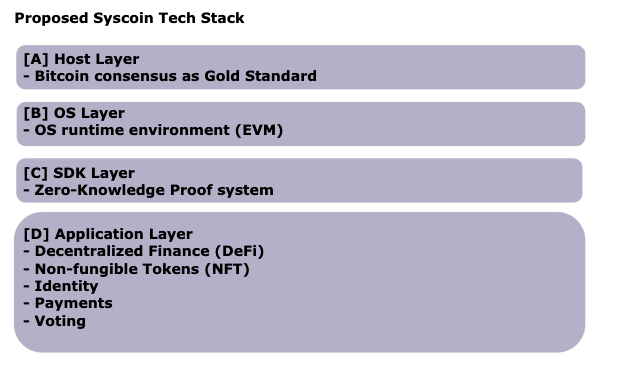
\includegraphics[width=3in]{img/tech_stack.png}
\label{fig:tech_stack}
\caption{sys tech stack} 
\end{figure} 

Surprisingly, these ideals represent a design that is not shared with any other project in the industry, including Bitcoin or Ethereum. We recommend that these ideals, fashioned together in a singular protocol, could possibly present a grand vision for a “World Computer” blockchain infrastructure.

Syscoin has already implemented Geth + Syscoin nodes in one application instance already (ie, release 4.2), we foresee that there will not be any challenges associated with building a consensus basis working together to form a dual chain secured by Syscoin’s PoW.

Fig 5 describes a system where nodes are running two sets of software processes, the Syscoin chain protocol and an EVM/eWASM chain protocol which are kept in sync through putting the EVM tip hash into the Syscoin block. Both have their own individual mempools and effectively the Ethereum contracts, tools and processes can directly integrate as is into the EVM chain as it stands. Note that the two chains are processes running on the same computer together. Thus a SYS NODE and EVM NODE would be operating together on one machine instance (ie, Masternode) with ability to communicate with each other directly through Interprocess Communication (IPC). The intersection between the two processes happens in three points:

\begin{enumerate}
\item Miner of the EVM chain collects the latest block hash and places it into the Syscoin block.
\item When validating Syscoin blocks, nodes confirm the validity of the EVM tip by consulting the EVM chain software locally
\item Fees for the EVM chain are to be paid in SYS. We need an asset representing SYS on the EVM chain, which will be SYSX. We will enable this through a similar working concept that we’ve already established (SysEthereum Bridge). We may also enable pre-compiles on the EVM chain side to extract Syscoin block hashes and merkle roots to confirm validity of SYS to SYSX burn transactions.
\end{enumerate}

As seen in Fig 6, work done on BTC is reused to create SYS blocks through the merged-mining specification. Concurrently, the miner will execute smart contracts in the memory pool of the node running the EVM chain. Once a chain hash has been established post-execution, it will be put into the coinbase of the Syscoin block and published to the network. Upon receiving these blocks, every node would verify that the EVM chain which can be locally executed (ie, similar to the miner) matches the state described by the Syscoin block. Technically, one would want to ensure both the latest and previous EVM block hashes inside of their respective Syscoin blocks are valid. The block $->$ evmblock $==$ evmblock \&\& block $->$ prev $==$ evmblock $->$ prev is all that is needed to link the chains together with work done by Bitcoin which is propagated to Syscoin through AUXPOW and can serve as a secure ledgering mechanism for the EVM chain.

Since (a) we may use eWASM; (b) there are paid full nodes running on the network; and (c) the mining costs are shared with Bitcoin miners, we should be able to safely increase the amount of bandwidth available in the EVM chain while remaining secure from large uncle orphan rates. There has been much discussion as to what the safe block size should be on Ethereum. Gas limits are increasing as optimizations are made on the Ethereum network. However, since this network would be ledgered by the Syscoin chain through PoW, there shouldbe no concern for uncle orphaning of blocks since the blocks must adhere to the policy set inside of the Syscoin block. We should therefore be able to increase bandwidth significantly and parameterize for a system that will scale globally yet still be centered around L2 rollup designs. A very important distinction to note is that the design of Ethereum 2.0 centers around a Beacon chain and sharding served by a Casper consensus algorithm \cite{But17}. The needs of the algorithm require a set of finality guarantees necessitating a move towards Proof-of-Stake (PoS). This has large security implications for which we may not have formal analysis for a long time, however we do know it comes with big risk \cite{Neu21}.  We offer similar levels of scalability on a network while retaining Nakamoto Consensus security. The simpler design which has been market tested and academically verified to work would result in a more efficient system as a whole with less unknown and undocumented attack vectors. The only research that would need to be made therefore is on the optimal parameterization of the gas limit taking into account an L2 centric system but also a safe number of users we expect to be able to serve before fee market mechanisms begin to regulate the barrier of entry for these users. This proposed system should be scalable enough to serve the needs of global generalized computation while sticking to the core fundamentals set forth in the design ideals above. Our upcoming whitepaper will have more analysis on these numbers but we will include some theoretical scaling metrics at the end of this article.

\subsubsection{Related Works}


The following organizations offer various open source third party L2 scaling solutions:

\begin{itemize}
\item ZEXE(Aleo)
\item Starkware
\item Matter labs
\item Hermez
\item Connext
\end{itemize}

Starkware is built using a general purpose language (Cairo) with Solidity (EVM) in mind, as is Matter labs with the (Zinc) language. Hermez developed custom circuits tailor-suited to fast transactions and Decentralized Exchange (DEX) like capability. These will be able to directly integrate into Syscoin without modification. As such, the optimizations and improvements they make should directly be portable to Syscoin, hence becoming partners to our ecosystem.

Aleo uses Zero knowledge EXEcution (Zexe) for zkSNARK proof creation through circuits created from R1CS constraints. The interesting thing about Aleo is that there is a ledger itself that is purpose-built to only verify these Zexe proofs for privacy preserving transactability. The consensus is PoW, while the proof system involves optimizing over the ability to calculate the verifications of these proofs efficiently. The more efficient these miners become at verifying these proofs, the faster they are able to mine and thus the system provides sybil resistance through providing resources to verify Zexe proofs as a service in exchange for block creation. However, these proof creations can be done in parallel based on the business logic for the systems the developers need to create. There is no direct need for on-chain custom verification as these can be done in an EVM contract, similar to what Cairo Generic Proving Service (GPS) verifier and Zinc Verification do. The goal of Aleo is to incentivize miners to create specialized hardware to more efficiently mine blocks with verification proofs. However, provers can also do this as we have seen with Matter Labs’ recent release of FPGA to do more efficient zkSNARK proofs \cite{Glu20}. It is a desirable property to use PoW to achieve “world-view” consensus in Aleo; however they focus on private transactions. They are typically not batched and employ a recursive outer proof to guarantee execution of an inner proof where the outer proof is sent to the blockchain to be verified. This proof is a limited 2-step recursion, consequently batching of arbitrary amounts of transactions is not supported. However, as a result the cost of proof verification is relatively constant with a trade-off of limiting the recursion depth. Aleo is not meant to be a scalable aggregator of transactions, but mainly oriented towards privacy in their zk-SNARK constructions using Zexe.


\subsubsection{Functional Overview}

For scalable simple payments, one can leverage our Syscoin Platform Token (SPT) asset infrastructure and payment channels to transact at scale. Unique characteristics of SPTs include a generalized 8 byte field for the asset ID which is split between the upper and lower 4 bytes; the upper 4 are issued and definable (ie, NFT use cases) and lower 4 are deterministic. This enables the ability to have a generalized asset model supporting both Non-fungible Tokens (NFT) and Fungible Tokens (FT) without much extra cost at the consensus layers. 1 extra byte is used for all tokens at best case and 5 extra bytes are used for NFT at worst case. See \cite{NFT21} for more information on Syscoin’s NFTs. This model promotes multiple assets to be used as input and consequently as outputs, suggesting that  atomic swaps between different assets are possible within 1 transaction. This has some desirable implications when using payment channels for use cases such as paying in one currency when merchants receive another atomically. A multi-asset payment channel is a component that is desired so users are not constrained to single tokens within a network. Composability of assets as well as composability across systems (such as users from one L2 to another) is a core fundamental to UX and convenience that needs to be built into our next generation blockchain components that we believe will enable mass adoption. The Connext box shows how potentially you can move from one L2 on one network to another as described in \cite{Bhu21}. This would promote seamless cross-chain L2 communication without the high gas fees. Since these L2’s are operating under an EVM/eWASM model, there are many ways to enable this cross-communication.

An EVM layer will support general smart contracts compatible with existing Ethereum infrastructure and L2 rollups will enable massive scale. The different types of zkRollups will allowbusinesses and rollup providers to offer ability for custom fee markets (ie, pay for fees in tokens other than base layer token SYS). In addition, it will remove costs and thus improve scale of systems by offering custom data availability consensus modules. This design discussed here shares similarities to the zkPorter design where a smart contract would sign off on data availability checks that would get put into the ZKP as part of the validity of a zkBlock which goes on chain.

The overall idea of the zkPorter design is that the zkRollup system would be called a “shard”, and each shard would have a type either operating in “zkRollup” mode or operating in “normal” mode. 

This concludes that shards can define different consensus modules for data availability (censorship resistance mechanisms) via separating concerns around ledgering the world-view of the state (ie, ZKP that is put on L1 and the data that represents the state. Doing so would allow shards to increase scale, offload costs of data availability to consensus participants.

A few note-worthy examples of consensus for data availability are:

\begin{enumerate}
\item Non-committee, non fraud proof based consensus for data availability checks. No $2/3$ online assumption; see ethresear.ch post \cite{But20}. 
\item Sublinear block validation of ZKP system. Use something like Lazy Ledger as a data availability proof engine and majority consensus; see ethresear.ch post \cite{Al20}. 
\item Use a combination of above, as well as masternode quorum signatures for any of the available quorums to sign a message committing to data availability checks as well as data validity. Using masternodes can provide a deterministic set of nodes to validate decisions as a service. The data can be stored elsewhere accessible to the quorums as they reach consensus that it is indeed valid and available.
\end{enumerate}


\begin{figure}[h!]
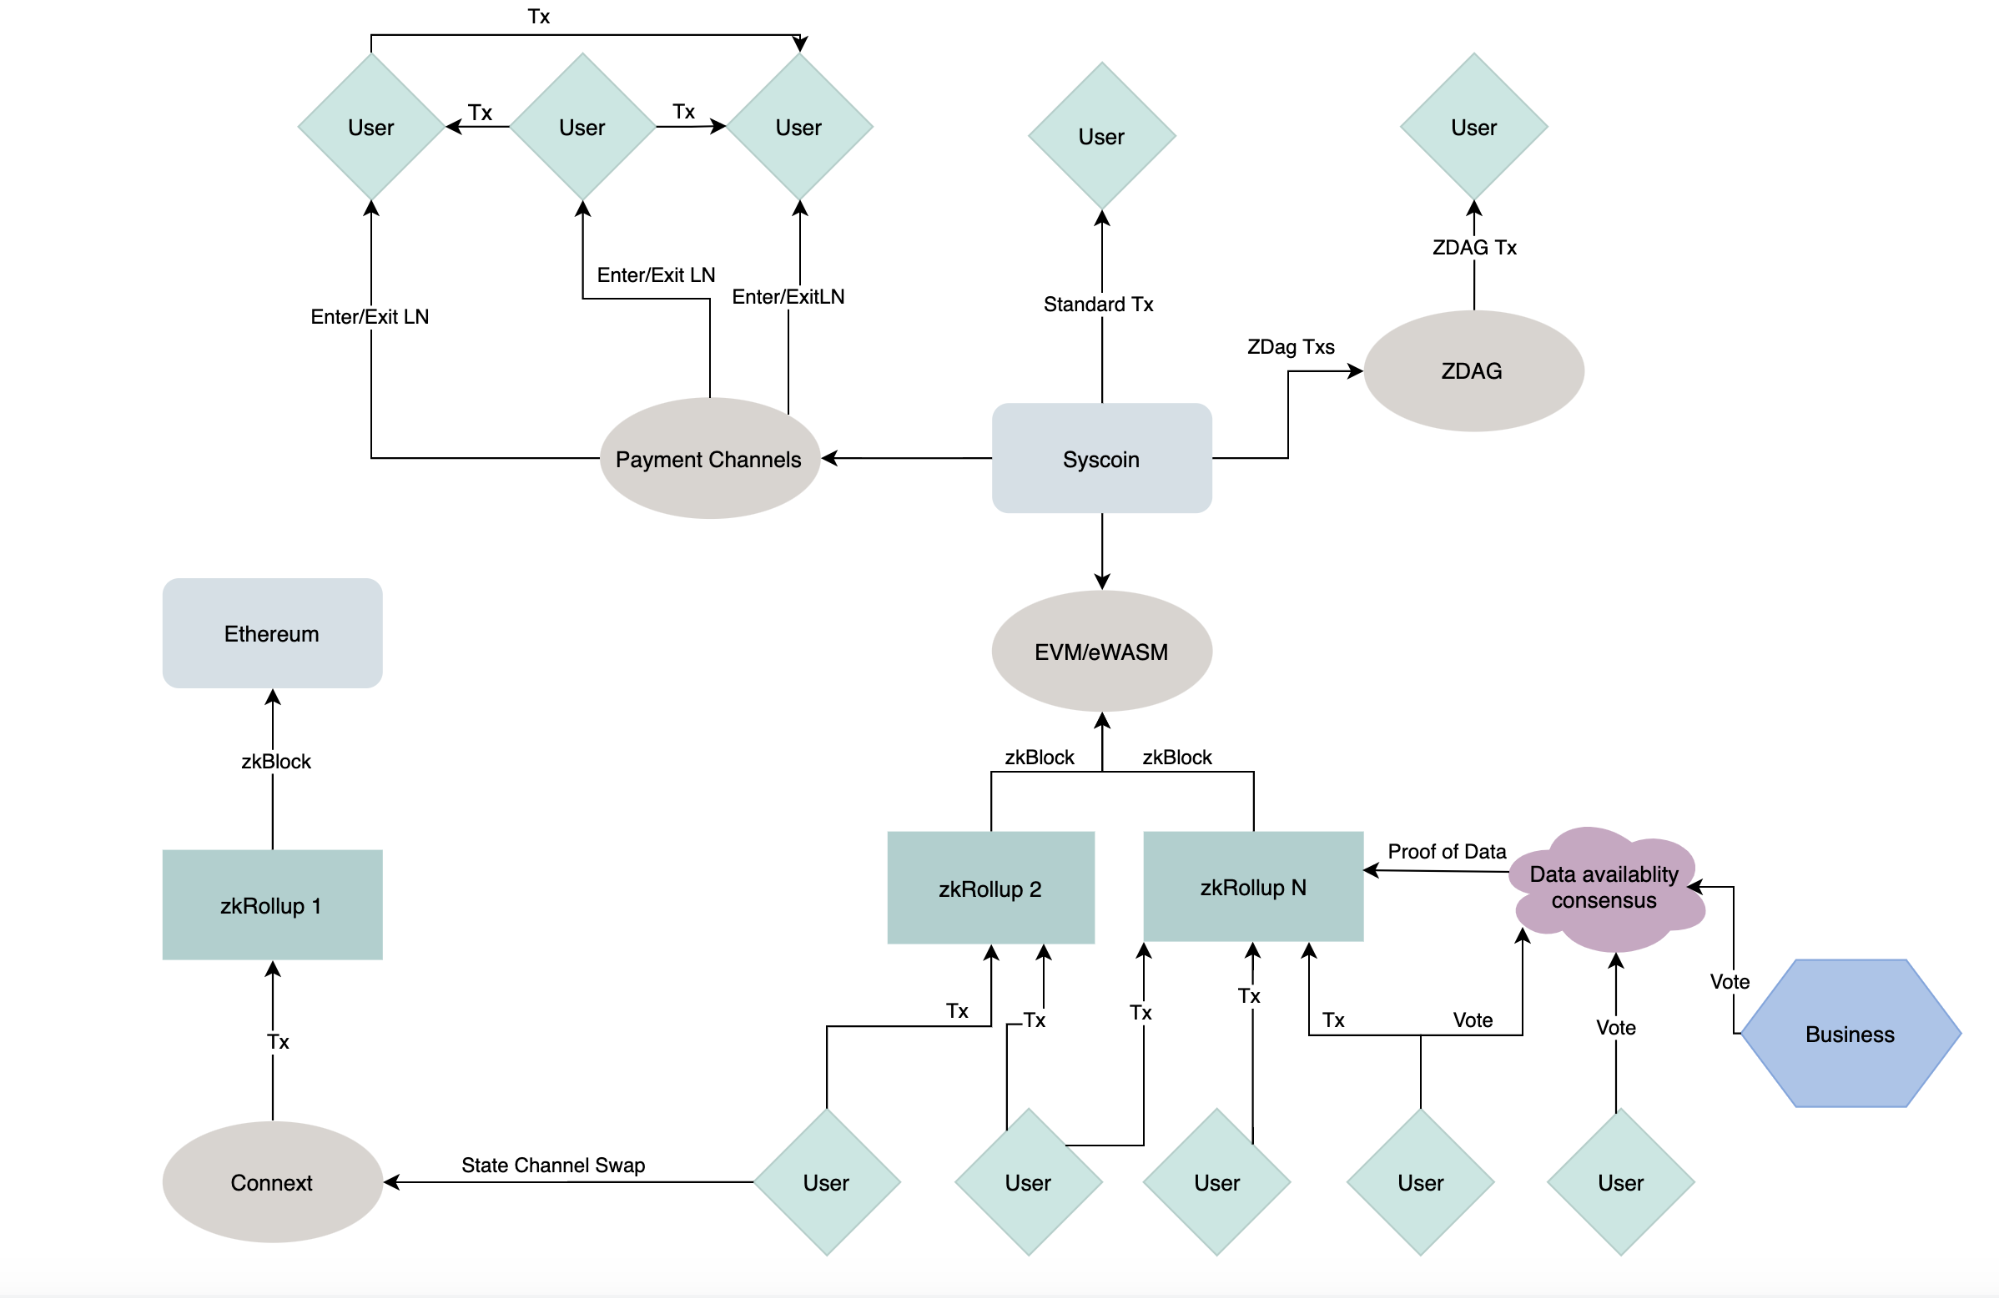
\includegraphics[width=3in]{img/nevm.png}
\label{fig:nevm}
\caption{Network EVM: High level description} 
\end{figure} 

\subsubsection{Optimistic vs ZkRollup}

ZKP are excellent for complex calculations above and beyond simple balance transfers. For payments, we feel UTXO payment channels combined with something like Z-DAG is an optimal solution. However, we are left with rollup solutions for generalized computation involving more complex calculations requiring consensus.

The solution we adopt has to be secured by L1 consensus that is considered decentralized and secure, which we achieved via merged-mining with Bitcoin.

There are two types of rollup solutions today: (a) Optimistic roll ups (OR); and (b) zkRollups; which offer trade-offs.

Consensus about which chain or network you are working on is a difficult problem that is solved for us by Nakamoto consensus. We build on that secure longest chain rule (supplemented by Chain Locks to prevent selfish mining) to give us the world-view of the rollup states. The executions themselves can be done once by a market of provers, never to be re-executed, only verified, suggesting it  becomes an almost constant cost on an arbitrarily large number of executions batched together. With OR you have the same world-view but the world-view is editable without verifying executions. The role of determining the validity of that world-view is delegated to someone watching who provides guarantees through crypto-economics. Zero-knowledge proofs remove crypto-economics on execution guarantees and replace them with cryptography.

See \cite{Sta19} to see contrasting benefits between fraud proofs (optimistic) vs validity proofs (zk). Key takeaways from this article are as follows:

\begin{itemize}
\item Eliminate a nasty tail risk: theft of funds from OR via intricate yet viable attack vectors;
\item Reduce withdrawal times from 1–2 weeks to a few minutes;
\item Enable fast tx confirmations and exits in practically unlimited volumes;
\item Introduce privacy by default.
\end{itemize}

An area that has been overlooked is interoperability. A generalized form of cross-chain bridging can be seen in Chain A locking tokens based on a preimage commitment by Chain B to create a zero-knowledge proof, followed by verification of that proof as the basis for manifesting equivalence on Chain B. Any blockchain with the functionality to verify these proofs could participate in the ecosystem.

Our vision here is described using a hzkRollup centric world-view, yet it can be replaced with other technologies should they be able to serve the same purpose. As an infrastructure we are not enforcing one or the other as developers can build on what they feel best suits their needs. We believe we are close to achieving this, and that the technology is nearing the point of being ready for the vision set forth in this article.


\subsection{Evidence}

Simple payments: since payment channels work with UTXO’s and also benefit from on-chain scaling via Z-DAG, 16MB blocks (with segwit weight) assumed, we will see somewhere around 8MB-12MB effectively per minute (per block). We foresee that is sufficient to serve 7 Billion people who may enter and exit the payment channel networks once a year (ie, 2 transactions on chain per person per year) for a total of 14 Billion transactions. Let’s conservatively assume 8MB blocks and 300 bytes per transaction. Once on a payment channel, the number of transactions is not limited to on-chain bandwidth, but to network related latencies and bandwidth costs. Therefore, we will conclude that our payment scalability will be able to serve billions of people doing 2 on-chain transactions per year which is arguably realistic based on the way we envision payments to unfold; whether that is an L2 or payment channel network that will hold users to pay through instant transaction mechanisms. On-chain, we have some metrics on Z-DAG throughput [1]; in those cases someone needs to transact for point-of-sale using the Syscoin chain. The solution for payments ends up looking like a hybrid mechanism of on-chain (Z-DAG) and off-chain (ie, payment channel) style payments.

Complex transactions such as smart contracts using zkRollups require a small amount of time to verify each proof. In this case, we assume that we will host data off-chain while using an off-chain consensus mechanism to ensure data availability for censorship resistance; so the only thing that goes on the chain are validity proofs. We will assume that we will assign 16MB blocks for the EVM chain per minute. 

A proof size will be about 300kB for about 300k transactions batched together which will take about 60-80ms to verify and roughly 5 to 10 minutes to create such proofs. These are the Reddit bake-off estimates using zk-STARKs which present quantum resistance and no trusted setup. After speaking with Eli Ben-Sasson, we were made aware that  proving and verifications metrics are already developed compared to  what is  currently presented by Starkware \cite{Sta20}. Hence, zk-SNARKs offer even smaller proofs and verification times at the expense of trusted setups and stronger cryptography assumptions (not post-quantum safe). We foresee that these numbers will improve over time as the cryptography improves, but current estimates suggest a rough theoretical capacity of around 1 Million TPS. 

Starkware was able to process 300k transactions over 8 blocks with a total cost of 94.5M gas; final throughput was 3000 TPS (see Reddit bake-off estimates). As a result, or the following calculations, let’s assume one batch-run to be 300k transactions.
Ethereum can process ~200kB of data per minute, with a cost limit of 50M gas per minute. Therefore, considering the Starkware benchmark test, and assuming a block interval of 13 seconds, we would achieve ~ 3000 TPS (ie,  300 k transactions per batch-run / (8 blocks per batch-run * 13 seconds per block))

It is estimated that Syscoin will be able to process ~16MB of data per minute on the EVM layer (ie, SYSX in Fig 3), which is ~80x gain over Ethereum; thus a cost limit of 4B gas (ie, 80*50M) per minute. Therefore, if the Starkware benchmark test was run on Syscoin, it is estimated that Syscoin could run the equivalent of 42 batch-runs per minute (ie, 4B gas per minute / 94.5 M gas per batch-run). That would result in an equivalent of 210 k TPS (ie, 42 batch-runs per minute * 300 k transactions per batch-run / 60 seconds per minute).

If we were to consider using Validum on the Syscoin EVM layer, we estimate that we could achieve 800 batch-runs per minute (ie, 4B gas per minute / 5 M gas per batch-run). That would equate to an equivalent of 4M TPS (ie, 800 batch-runs per minute * 300 k transactions per batch-run / 60 seconds per minute).

\textbf{Table 1}

Because of the higher throughput capabilities of baseline EVM, we may look to dynamically adjust costs of the gas limits \cite{Che17} to thwart DOS attacks.

The aforementioned calculations demonstrate the full State Safety of the mainchain secured by Bitcoin, and no asynchronous network assumptions which make theoretical calculations impractical in many other claims of blockchain throughput due to execution model bottlenecks. These results were extrapolated based on real results with constant overhead added that becomes negligible with optimizations. It is imperative to  note that transactions in this strategy are not re-executable; there is little to no complexity in this model other than verifying succinct proofs. The proof creation strategy is parallelized organically using this model. The verifications on the main chain can also be parallelized as they are executed on separate shards or rollup networks. Dual parallel execution and verification gives exponentially more scalability than other architectures. Additionally, privacy can be built into these models at minimal to no extra cost, depending on the business model. Lastly, we suggest  these are sustainable throughput calculations and not burst capacity numbers which would be much higher (albeit with a marginally higher fee based on fee markets). For example Ethereum is operating at 15 TPS but there are around 150k transactions pending, and the average cost is about 200 gWei currently. The fee rate is based on the calculation that it  takes around 10000 seconds to clear, assuming this many transactions, no new transactions, and there is demand to settle earlier. Extrapolating on 4M TPS the ratio would become 40B transactions pending with 4M TPS to achieve the same fee rate on Ethereum today assuming the memory pool is big enough on nodes to support that many pending transactions. Since masternodes on Syscoin are paid to provide uptime, we can expect network bandwidth to scale up naturally to support higher throughput as demand for transaction settlement increases. Today, the ability to transact at a much higher rate using the same hardware provides the ability for a greater scale than the state-of-the-art in blockchain design without the added desired caveat of avoiding asynchronous network assumptions. We believe this proposed design will become the new state-of-the-art blockchain, which is made viable due to its security, flexibility and parallelizable computational capacity.

In regards to uncle rates with higher block sizes, keep in mind we make uncle rates and re-organizations in general negligible through the use of the PoW chain mining Syscoin along with Chain Locks. We provide intuition that block sizes can be increased substantially without affecting network health. Furthermore, the gas limits can be adjusted by miners up to 0.1\% from the previous block and so a natural equilibrium can form where even if more than 4B gas is required it can be established based on demand and how well the network behaves with such increases. There is a lot to unpack with such statements and so we will cover this in a separate technical post as it is out-of-scope for this discussion.

\begin{figure}[h!]
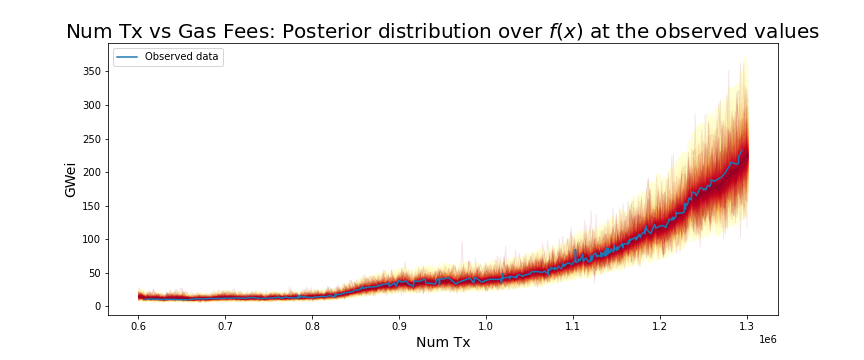
\includegraphics[width=3in]{img/eth_tx_vs_gas.png}
\label{fig:eth_tx_vs_gas}
\caption{eth tx vs gas} 
\end{figure} 

\begin{figure}[h!]
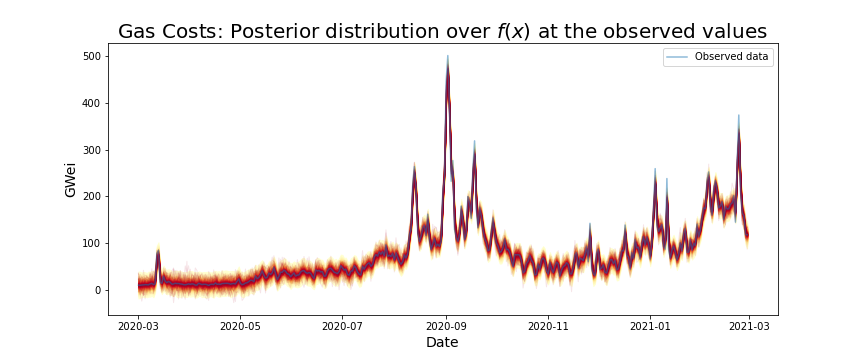
\includegraphics[width=3in]{img/eth_gas_costs.png}
\label{fig:eth_gas_costs}
\caption{eth gas costs} 
\end{figure} 

\begin{figure}[h!]
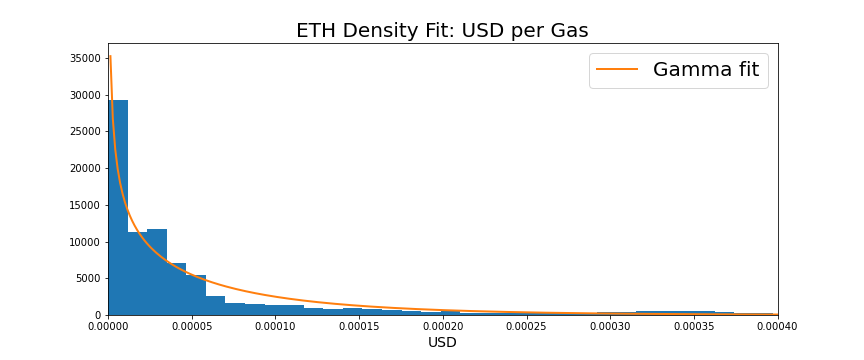
\includegraphics[width=3in]{img/eth_usd_density.png}
\label{fig:eth_usd_density}
\caption{eth usd density} 
\end{figure} 

\begin{figure}[h!]
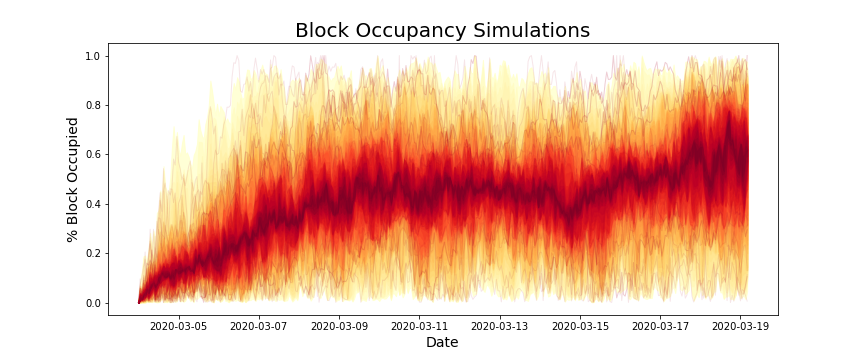
\includegraphics[width=3in]{img/blk_occupancy_simulations.png}
\label{fig:blk_occupancy_simulations}
\caption{sysx blk occupancy simulations} 
\end{figure} 

\begin{figure}[h!]
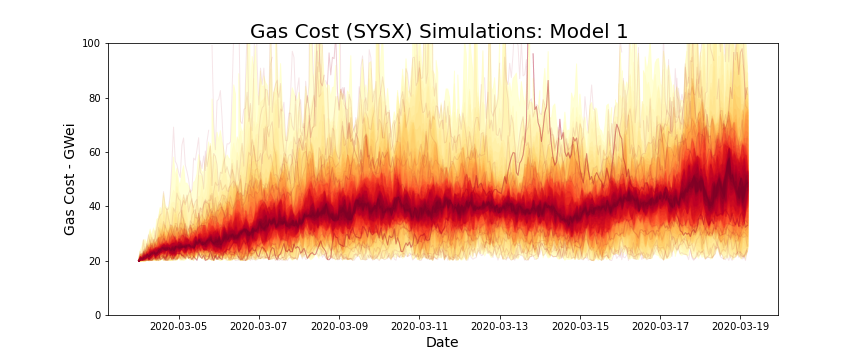
\includegraphics[width=3in]{img/sysx_gas_costs_m1.png}
\label{fig:sysx_gas_costs_m1}
\caption{sysx gas cost simulations} 
\end{figure} 

\begin{figure}[h!]
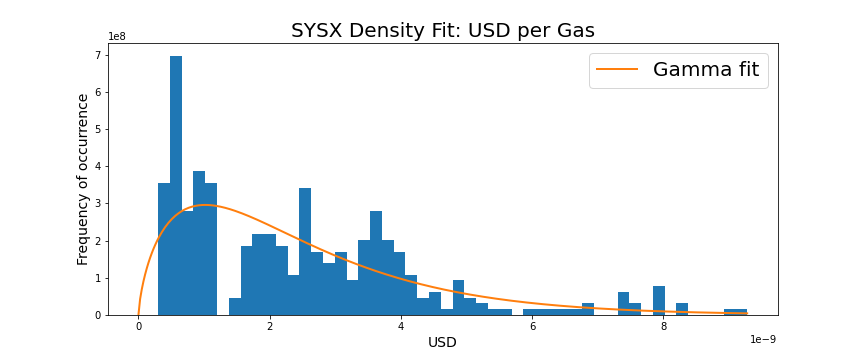
\includegraphics[width=3in]{img/sysx_usd_density.png}
\label{fig:sysx_usd_density}
\caption{sysx usd density} 
\end{figure} 



\subsubsection{Decentralized Cost Model}

Decentralized cost models lead to exponential efficiency gains in economies of scale. We set forth a more efficient design paradigm for execution models reflective of user intent. This design uses the UTXO model to reflect simple state transitions and a ZKP system for complex computations leading to state transitions. This leads to ideal scalability for a system by allowing people to actively make their trade-off within the same ecosystem, driven by the same miners securing that ecosystem backed by Bitcoin itself.

Furthermore, a decentralized cost model contributes to scalability in that ZKP gates can generalize complex computation better than fee-market resources like gas or the CPU/memory markets of EOS, etc. This results in leads to more deterministic and efficient consumption of resources maximizing efficiency in calculations, and gives opportunity for those to scale up or down based on economic incentives without creating monopolistic opportunities unlike ASIC mining. In other words, the cost is dictated by what the market can offer, via the cost of compute power (as dictated by Moore's law) instead of constrained costs of doing business on the blockchain itself. This model could let the computing market dictate the price for Gas instead of being managed by miners of the blockchain. The miners would essentially only dictate the costs of the verification of these proofs when they enter the chain rather than the executions themselves.

We can already begin to see computational optimization through hardware happening with ZKP and with a decentralized cost model it will be much simpler to understand costs of running prover services as well as know how the costs scale based on the number of users and parameters of systems that businesses would like to employ. All things considered, it will be more efficient to make accurate decisions on data availability policies and the consensus systems needed to keep the system censorship resistant and secure.

Rollups will be friends, that is, users of one rollup system doing X TPS and users of another doing Y TPS, with the same trust model, will in effect get us to global rates of X*Y (where X is TPS of the sidechains/rollups and Y is the number of sidechains and rollups that exist). X is fairly static in that the execution models of rollups do not change drastically (and if they do, the majority of those rollup or sidechain designs end up switching to the most efficient design for execution over time).


\begin{table*}[h!]
\centering
\begin{tabular}{ |c|c|c|c|c|c|c|c|c|c|   } 
\hline
Chain & Gas  Limit & Block Time & Mode & Cost  & Amortized  & Total TPS & \multicolumn{3}{|c|}{USD / 300K Tx (Mar 20 to Mar 21) } \\
 &  &  &  &  300K Tx  & Cost per Tx  &  & median & lwr 5\% &  upr 95 \% \\ 
\hline
\multirow{3}{*}{ETH} & \multirow{3}{*}{12.5M} & \multirow{3}{*}{13 sec} & L1 & 6.3B gas  & 21,000 gas  & ~45 & 159,328.24 & 10,669.40  & 1,914,394.79  \\ 
\multirow{3}{*}{} & \multirow{3}{*}{} & \multirow{3}{*}{} & L2 zk-Rollup & 94.47M gas  & 315 gas & ~3,000* & 2,389.16 & 159.99  & 28,706.81 \\ 
\multirow{3}{*}{} & \multirow{3}{*}{} & \multirow{3}{*}{} & L2 Validium  & 5M gas  & 17 gas & ~56,000** & 126.45 & 8.47  & 1,519.36 \\ 
\hline

\multirow{3}{*}{SYSX} & \multirow{3}{*}{4B} & \multirow{3}{*}{60 sec} & L1 & 6.3B gas  & 21,000 gas  & ~3,100*& 9.31453 & 1.76308 & 37.01621 \\ 
\multirow{3}{*}{} & \multirow{3}{*}{} & \multirow{3}{*}{} & L2 zk-Rollup & 94.47M gas  & 315 gas & ~210,000** & 0.13967 & 0.02644  & 0.55507 \\ 
\multirow{3}{*}{} & \multirow{3}{*}{} & \multirow{3}{*}{} & L2 Validium  & 5M gas  & 17 gas & ~4,000,000 & 0.00739 & 0.00140  & 0.02938 \\ 
\hline

\end{tabular}
\caption{Comparison of Gas and USD costs between ETH and SYSX}
\label{table:1}
\end{table*}


\subsection{Applications}

Commercial enterprises may start to create proprietary prover technologies where costs will be lower than market in an attempt to create an advantage for user adoption. This design is made possible since the code for the prover is not required for the verifier to ensure that executions are correct. The proof is succinct whether or not the code to make the proof is available.

While  the barrier of entry is low in this industry, we’ve seen the open source model and its communities optimize hardware and software and undergo academic peer review using strategies  that outpace private funded corporations. That is plausible to play out over the long term. However, an organic market will likely form on its own, forging its own path leading to mass adoption through capitalist forces. The point here is that the privately funded vs open source nature of proving services does not change the mechanism of secure and scalable executions of calculations that are eventually rooted to decentralized and open ledgers secured by Bitcoin.

The utmost interesting propositions are the verticals that become possible by allowing infrastructure that is parameterized to scale into those economies where they are needed most, and where trust, security and auditability of value are concerns. Smart cities, IoT, AI and Digital sovereignty are large markets that intersect with blockchain as a security blanket. Although ZKP are tremendously useful on their own, applying them to consensus systems for smart contract executions drive them to another level due to the autonomous nature of “code-is-law” and provable deterministic state of logic. We believe a large majority of the next generation economy will depend on many of the ideas presented here. Blockchain Foundry is working with commercial and enterprise adopters of blockchain technology. Our direct interaction with clients combined with our many collective years of experience in this field are reflected in this design.


\section{Specifications}
\label{section:specs}


General specifications for Syscoin 4.0:

\begin{description}[font=$\bullet$~\normalfont\scshape\color{blue!50!black}]
\item \textbf{Max Coins:} 888 Million
\item \textbf{Deflation:}  5 percent per year until Max Coins
\item \textbf{Consensus:} PoW/PoS Hybrid. PoW is SHA256
Merge-mined with Bitcoin
\item \textbf{Block time:} 60 seconds 
\item \textbf{Rewards:} 38.5 Syscoin deflated 5 percent per year
of which 10 percent is allocated to governance proposals (3.85 Syscoin). 75 percent of the result goes
to masternode and 25 percent to miner.
\item \textbf{Difficulty algorithm:} Dark Gravity Wave
\item \textbf{Masternode collateral requirement:} 100000 Syscoin
\item \textbf{Masternode seniority}: 3 percent every 4 months until
27 percent over 3 years
\item \textbf{Governance proposals payout schedule}: every month
\item \textbf{Governance funding per round}: 168630 Syscoin per
month
\end{description}


\section{Conclusion}
\label{section:conclusion}
Praesent mauris. Fusce nec tellus sed augue semper porta. Mauris massa. Vestibulum lacinia arcu eget nulla. Class aptent taciti sociosqu ad litora torquent per conubia nostra, per inceptos himenaeos. Curabitur sodales ligula in libero. Sed dignissim lacinia nunc. Curabitur tortor. Pellentesque nibh. Aenean quam. In scelerisque sem at dolor. Maecenas mattis. Sed convallis tristique sem. 

\appendices

\section{Security: PoW vs PoS}

Proof of Stake (PoS) systems have security threats that are not inherent in Proof of Work (PoW) systems as outlined in Table \ref{table:pow_vs_pos}, of which Bitcoin employs. Hence, PoS is less secure than PoW. In terms of security, we call the Bitcoin PoW protocol the gold standard, which is the same security mechanisim that Syscoin uses.

\begin{table}[h!]
\centering
\begin{tabular}{ |c|c|c|c| } 
\hline
 & \multicolumn{3}{|c|}{ Vulnerability } \\
 Attack type & PoW & PoS & Delegated PoS \\
\hline
Short range attack & - & + & - \\
Long range attack & - & + & + \\
Coin age accumulation attack & - & maybe & - \\
Precomputing attack & - & + & - \\
Denial of service & + & + & + \\
Sybil attack & + & + & + \\
Selfish mining & maybe & - & - \\
\hline
\end{tabular}
\caption{Comparing PoW to PoS consensus mechanism; plus sign (+) indicates vulnerability; see \cite{Bit15}. As shown, PoW system has the least number of vulnerabilities}
\label{table:pow_vs_pos}
\end{table}

\section{ZDAG Fundamentals}

Zero-Confirmation Directed Acyclic Graph (ZDAG) is an instant settlement protocol that solves the 'fast-transaction' problem. It functions by using a directed acyclic graph (DAG) where validating nodes verify the sequential ordering of transactions that are received in their memory pools. More specifically, Syscoin approach is centred around the verification of signatures and relaying of transactions. It does this by prioritizing the relay of transactions over signature verification and recipient receives funds faster; see Table \ref{fig:dag_tx}. For algorithm see Appendix A in \cite{Sidb18} for the verification process.

\begin{figure}[h!]
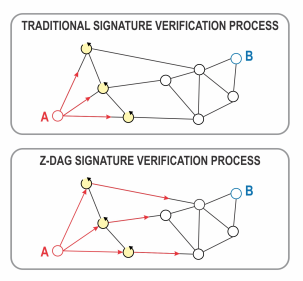
\includegraphics[width=3in]{img/dag_tx.png}
\caption{Traditional blockchain networks require each node to first check the signatures of incoming transactions before relaying them; this blocking technique bottlenecks broadcasting speed. The Z-DAG process as displayed above immediately relays transactions before checking signatures, resulting in significantly faster movement across the network} 
\label{fig:dag_tx}
\end{figure} 


\subsection{Transmission Path}

The expected number of common peers between k Masternodes is:

\begin{equation}
E\{cp_{k}\} = pk -m \left(1 - \left(1 - \frac{p}{m}\right)^{k}\right),
\end{equation}
where $p$ is the number of common peers, and $X_{i}$ is 1 when the $i^{th}$ masternode is a common peer and 0 otherwise. The probability of having $n$ common peers is given by: 

\begin{equation}
P(|cp| = n) = \frac{\binom{M}{c} \binom{M-c}{p-c} \binom{M-p}{p-c} }{\binom{M}{p}}
\end{equation}

\subsection{Transmission Delay}

Using a dataset (containing 2086 samples) of average transmission times of ten transmissions between two hosts, it was modelled using the Gamma distribution as shown in Figure \ref{fig:tx_delay}. Using this model, the probability of transmission arriving in a given time can be estimated at various time points.

\begin{figure}[h!]
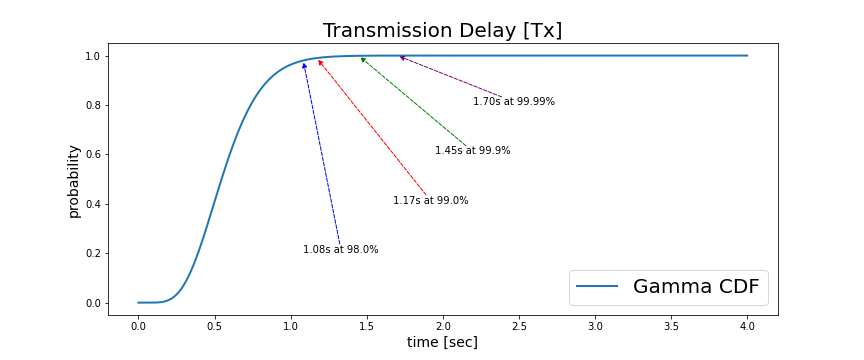
\includegraphics[width=3in]{img/transmission_delay.png}
\caption{Probability of Tx arrival after $5$ hops modelled via $X \sim Gamma(7.358,0.0777)$} 
\label{fig:tx_delay}
\end{figure} 

\section{Zero Knowledge Proofs Fundamentals}

The motivation of a Zero Knowledge Proof (ZKP) is to allow for one party (ie, prover) to convince another party (ie, verifier) of facts without revealing information (ie, zero knowledge). An example of a ZKP would be: allowing a subscriber (ie, prover) to gain access to an online service (ie, verifier) without revealing any personal data, other than the fact than that party is a paid subscriber.

A ZKP must satisfy three conditions:

\begin{enumerate}
\item \textbf{Completeness:} If statement is true, verifier will be convinced by prover
\item\textbf{Soundness:} If statement is false, a cheating prover cannot (except with some small probability) convince verifier it is true
\item \textbf{Zero-knowledge:} If statement is true, verifier knows nothing else
\end{enumerate}

\begin{figure}[h!]
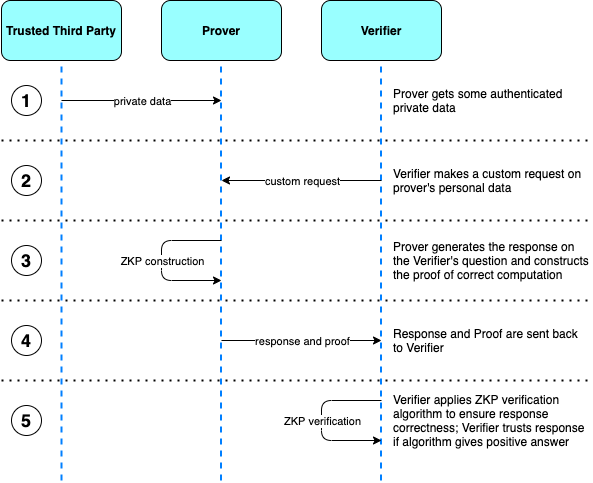
\includegraphics[width=3in]{img/zkp.png}
\caption{Data exchange in a Zero-knowledge proof system} 
\label{fig:zkp}
\end{figure} 

There are two types of ZKP:

\begin{enumerate}
\item \textbf{Interactive ZKP:} Comprised of multiple challenge / response messages (commitment, challenge and response); requires a stable communication channel
\item \textbf{Non-interactive ZKP:} Only needs single message and is more efficient; can be run offline
\end{enumerate}
zk-SNARK and zk-STARKS are types of Non-interactive ZKP , where no interaction is required between prover and verifier.

\section{Block Occupancy Cost (BLOC) Function}

We considered two approaches to model the gas costs, $y_{c}$, using model 1:
\begin{equation}
y_{c} = \dfrac{1}{k}\log\left(\dfrac{1+x_{o}}{1-x_{o}}\right) + y_{0};
\end{equation}
and model 2:
\begin{equation}
y_{c} = \left| \dfrac{1}{k(x_{o}-1)} \right| + y_{c,0} - \dfrac{1}{k},
\end{equation}
where $x_{o} \in [0,1]$ is the block occupancy, $y_{c,0}$ is the base cost, and $k$ is an adjustable scaling term. We call $y_{c}$ the BLock Occupancy Cost (BLOC) function.

Other variants of $y_{c}$ can be utilized highlighting various characteristics. For instance, Model 1 has the characteristic of being less volatile, but with a higher expected base cost than Model 2.

\section{Block Occupancy and Gas Simulations}

To simulate arbitrary block occupancies, we use the Beta distribution:

 \begin{equation}
\textbf{x}_{o,t} \sim Beta(\alpha_{t},\beta_{t})
 \end{equation}
 where $t$ is time, and $\beta_{t} = 1-\alpha_{t}$
 
To exhibit slow upward growth over time for $\alpha_{t}$, we used a MinMax scaled ARIMA(0,1,1) model, otherwise known as a simple exponential smoothing model with growth, which is of the form:

\begin{equation}
\hat{\alpha'}_{t} = \mu + \alpha'_{t-1} - \theta_{1}\epsilon_{t},
\end{equation}
and then applied MinMax scaling to ensure $\alpha_{t} \in [0,1]$:
\begin{equation}
\hat{\alpha_{t}} = \dfrac{\alpha'_{t} - min(\alpha'_{t})}{  max(\alpha'_{t}) - min(\alpha'_{t}) }.
\end{equation}

Block Occupancy simulations, \textbf{x}$_{o,t}$, were fed into the BLOC function, to achieve a set of gas simulations, \textbf{y}$_{c,t}$, at each instance of time $t$.

\subsection{Marginal Likelihood}

Assume observed data, $y$, are the sum of a Gaussian Process (GP) and Gaussian noise, given by:

\begin{eqnarray}
y = f(x) + \epsilon \\
\epsilon \sim N(0,\Sigma) 
\end{eqnarray}
The unknown function, $f(x)$, is modelled as

\begin{equation}
f(x) \sim GP(\mu(x), k(x,x')),
\end{equation}
where $\mu(x)$ and $k(x,x')$ are the mean and covariance function respectively; the covariance function is often called the kernel function, and can take on several forms based on the structure of the input data, $x$. In this work, we use the Matern 5/2 kernel, which is of the form:

\begin{equation}
k(x,x') = \left( 1 + \dfrac{\sqrt{g(x,x')}}{\ell} + \dfrac{g(x,x')}{3\ell^2}\right)\exp\left[ \dfrac{g(x,x')}{\ell} \right]\ 
\end{equation}
where
\begin{equation}
	g(x,x') = 5(x-x')^2.
\end{equation}

For this work, we looked at observations, $y$, probabilistically, which can be determined via:
\begin{equation}
p(y|x) = \int p(y | f,x) p (f, |x) df;
\end{equation}
this is otherwise known as the marginal likelihood; from a Bayesian context, this may be referred to as the evidence, which is the normalizing part of Bayes rule. Typically, due to the computational complexity, this is the tough part in Bayesian analytics, so we use Markov Chain Monte Carlo (MCMC) sampling using the PyMC3 python package.  

\begin{thebibliography}{00}


\bibitem{Sida18} J. Sidhu, \textit{Syscoin 3.0: A Peer-to-Peer Electronic Cash System Built For Business Applications}, Blockchain Foundry Inc, Feb. 2018. Accessed on: Dec 2020. [Online]. Available: https://syscoin.org/$syscoin3_whitepaper.pdf$

\bibitem{Sidb18} J. Sidhu, E, Scott, and A. Gabriel, \textit{Z-DAG: An interactive DAG protocol for real-time crypto payments with Nakamoto consensus security parameters}, Blockchain Foundry Inc, Feb. 2018. Accessed on: Dec 2020. [Online]. Available: https://syscoin.org/$syscoin3_whitepaper.pdf$


\bibitem{Som15} Y. Sompolinsky, and A. Zohar, \textit{Secure High-rate Transaction Processing in Bitcoin}, Proc. 19th Int. Conf. Financial Cryptogr, Data Secur. (FC’20), Jan 2015, pp. 507-527

\bibitem{Bir20} G. Birmpas, E. Koutsoupias, P. Lazos, F.J. Marmolejo-Cossío, \textit{Fairness and Efficiency in DAG-Based Cryptocurrencies}, Proc. 24th Int. Conf. Financial Cryptogr, Data Secur. (FC’15), Jan 2015, pp. 507-527


\bibitem{Nor19} N. Word, \textit{UTXO vs Global State}, Nov. 2019. Accessed on: Jan 2021. [Online]. Available: https://word.site/2019/11/20/utxo-vs-global-state/

\bibitem{Szt15} P. Sztorc \textit{Nothing is Cheaper than Proof of Work}, Aug. 2015. Accessed on: Jan 2021. [Online]. Available: https://www.truthcoin.info/blog/pow-cheapest/

\bibitem{Eya18} I. Eyal, and E.G. Sirer, \textit{Majority is not Enough: Bitcoin Mining is Vulnerable}, \emph{Communications of the ACM}., vol. 61, no. 7, Jun. 2018.

\bibitem{Cao20} B. Cao, Z. Zhang, D. Feng, S. Zhang, L. Zhang, M. Peng, and
Y Li, \textit{Performance analysis and comparison of PoW, PoS and DAG based blockchains}, \emph{Digital Communications and Networks}., vol. 6, no. 4, Nov. 2020, pp 480-485

\bibitem{But20} V. Buterin, \textit{Using polynomial commitments to replace state roots}, Ethereum Research, Mar. 2020. Accessed on: Jan 2021. [Online]. Available: https://ethresear.ch/t/using-polynomial-commitments-to-replace-state-roots/7095

\bibitem{Bit15} G., \textit{Proof of Stake Versus Proof of Work. Technical Report}, BitFury Group, 2015. Accessed on: Jan 2021. [Online]. Available: http://bitfury.com/content/5-white-papers-research/pos-vs-pow-1.0.2.pdf 

\bibitem{Duf18} E. Duffield, and D. Diaz, \textit{Dash: A Payments-Focused Cryptocurrency}, Dash, Aug 2018. Accessed on: Jan 2021. [Online]. Available: https://github.com/dashpay/dash/wiki/Whitepaper


\bibitem{BitCore} \textit{Bitcoin Core FAQ, Compact Blocks FAQ}, Accessed on: Feb 2021. [Online]. Available: https://bitcoincore.org/en/2016/06/07/compact-blocks-faq/

\bibitem{Blo18} ] A. Block, \textit{Mitigating 51\% attacks with LLMQ-based ChainLocks}. Accessed on: Feb 2021. [Online], Nov 2018. Available: https://blog.dash.org/mitigating-51-attacks-with-llmq-based-chainlocks-7266aa648ec9

\bibitem{Val19} J. Valenzuela, Andreas Antonopoulos, \textit{Calls Dash Chain Locks “a Smart Way of” Preventing 51\% Attacks}. Aug 22, 2019. Accessed on: Feb 2021. [Online]. Available: https://dashnews.org/andreas-antonopoulos-calls-dash-chainlocks-a-smart-way-of-preventing-51-attacks/

\bibitem{Bon18} D. Boneh, M. Drijvers, and G. Neven, \textit{BLS Multi-Signatures With Public-Key Aggregation}, Mar 2018. Accessed on: Feb 2021. [Online]. Available: https://crypto.stanford.edu/~dabo/pubs/papers/BLSmultisig.html

\bibitem{Dra18} J. Drake. \textit{Pragmatic signature aggregation with BLS}, May 2018. Accessed on: Feb 2021. [Online]. Available:  https://ethresear.ch/t/pragmatic-signature-aggregation-with-bls/2105

\bibitem{Bow17} S. Bowe, \textit{BLS12-381: New zk-SNARK Elliptic Curve Construction}, Mar 2017. Accessed on: Feb 2021. [Online]. Available: https://electriccoin.co/blog/new-snark-curve/

\bibitem{Blo18}  A. Block, \textit{BLS: Is it really that slow?}, Jul 2018. Accessed on: Feb 2021. [Online]. Available: https://blog.dash.org/bls-is-it-really-that-slow-4ca8c1fcd38e

\bibitem{Rou17}  S. de la Rouvier. \textit{Interplanetary Linked Computing: Separating Merkle Computing from Blockchain Computational Courts}, Jan 2017. Accessed on: Feb 2021. [Online]. Available: https://media.consensys.net/interplanetary-linked-computing-separating-merkle-computing-from-blockchain-computational-courts-1ade201ecf8a

\bibitem{Ano18} Anonymous Kid, Why the fuck did Satoshi implement the 1 MB blocksize limit? [Online forum comment], Jan 2018, Accessed on: Feb 2021. [Online]. Available:  https://bitcointalk.org/index.php?topic=2786690.0

\bibitem{Zer21} \textit{Zero-Knowledge Proofs What are they, how do they work, and are they fast yet?} Accessed on: Feb 2021. [Online]. Available: https://zkp.science/

\bibitem{Ben18} E. Ben-Sasson, I. Bentov, Y. Horesh, and M. Riabzev, \textit{Scalable, transparent, and post-quantum secure computational integrity}, IACR Cryptol, 2018, pp 46 

\bibitem{Dry19} Dryja, T, Utreexo: A dynamic hash-based accumulator optimized for the bitcoin UTXO set, IACR Cryptol. ePrint Arch., 2019, p. 611.

\bibitem{Hot19} G.I. Hotchkiss, \textit{The 1.x Files: The State of Stateless Ethereum}, Dec 2019. Accessed on: Feb 2021. [Online]. Available:   https://blog.ethereum.org/2019/12/30/eth1x-files-state-of-stateless-ethereum/

\bibitem{Bow18} S. Bowe, A. Chiesa, M. Green, I. Miers, P. Mishra, H. Wu: \textit{Zexe: Enabling decentralized private computation}. Cryptology ePrint Archive, Report 2018/962 (2018). Accessed on: Feb 2021. [Online]. Available:  https://par.nsf.gov/servlets/purl/10175111

\bibitem{Nil20} A. Nilsson, P.N. Bideh, J. Brorsson, \textit{A survey of published attacks on Intel SGX}. 2020, arXiv:2006.13598

\bibitem{Nel18} C. Nelson, \textit{Zero-Knowledge Proofs: Privacy-Preserving Digital Identity}, Oct 2018. Feb 2021. Accessed on: [Online]. Available: https://www.slideshare.net/SSIMeetup/zeroknowledge-proofs-privacypreserving-digital-identity-with-clare-nelson

\bibitem{Bon19} D. Boneh, \textit{Discrete Log based Zero-Knowledge Proofs}, Apr 2019,  Accessed on: Feb 2021 [Online].  Available: https://www.youtube.com/watch?v=wB3DlND7KEw

\bibitem{Qua18} \textit{Quantum Computing’s Implications for Cryptography (Chapter 4)}, National Academies of Sciences, Engineering, and Medicine: Quantum Computing: Progress and Prospects. The National Academies Press, Washington, DC, 2018.

\bibitem{Nai19} S. Naihin, \textit{Goodbye Bitcoin… Hello Quantum}, Apr 2019, Accessed on: Feb 2021 [Online].   https://www.linkedin.com/pulse/goodbye-bitcoin-helloquantum-silen-naihin

\bibitem{Nas19} L.T. do Nascimento, S. Kumari, and V. Ganesan, \textit{Zero Knowledge Proofs Applied to Auctions}, May 2019, Accessed on: Feb 2021 [Online].   Available: https://courses.csail.mit.edu/6.857/2019/project/18-doNascimento-Kumari-Ganesan.pdf

\bibitem{But17} V. Buterin and V. Griffith, Casper the Friendly Finality Gadget. CoRR, Vol. abs/1710.09437, 2017. arxiv: 1710.09437, http://arxiv.org/abs/1710.09437

\bibitem{Neu21} M. Neuder, D.J. Moroz, R. Rao, and D.C. Parkes, \textit{Low-cost attacks on Ethereum 2.0 by sub-1/3 stakeholders}, 2021. arXiv:2102.02247,  https://arxiv.org/abs/2102.02247

\bibitem{Sta19} Starkware, \textit{Validity Proofs vs. Fraud Proofs}, Jan 2019, Accessed on: Feb 2021, [Online]. Available: https://medium.com/starkware/validity-proofs-vs-fraud-proofs-4ef8b4d3d87a

\bibitem{Glu20} A. Gluchowski, \textit{World’s first practical hardware for zero-knowledge proofs acceleration}, Jul 2020, Accessed on: Feb 2021 [Online]. Available:  https://medium.com/matter-labs/worlds-first-practical-hardware-for-zero-knowledge-proofs-acceleration-72bf974f8d6e

\bibitem{NFT21}  \textit{Introducing an NFT Platform Like No Other}, Accessed on: Feb 2021. [Online]. Available: https://syscoin.org/news/introducing-an-nft-platform-like-no-other

\bibitem{Bhu21} A. Bhuptani, \textit{Vector 0.1.0 Mainnet Release, The beginning of a multi-chain Ethereum ecosystem}, Jan 2021, Accessed on: Feb 2021.  [Online]. Available:  https://medium.com/connext/vector-0-1-0-mainnet-release-9496ae52c422

\bibitem{But20}  V. Buterin, \textit{With fraud-proof-free data availability proofs, we can have scalable data chains without committees}, Jan 2020, Accessed on: Feb 2021.  [Online]. Available:  https://ethresear.ch/t/with-fraud-proof-free-data-availability-proofs-we-can-have-scalable-data-chains-without-committees/6725

\bibitem{Al20} M. Al-Bassam,\textit{ A data availability blockchain with sub-linear full block validation}, Jan 2020, Accessed on: Feb 2021.  [Online]. Available:  https://ethresear.ch/t/with-fraud-proof-free-data-availability-proofs-we-can-have-scalable-data-chains-without-committees/6725

\bibitem{Che17}  T. Chen, X. Li, Y. Wang, J. Chen, Z Li, X. Luo, M. H. Au, and X. Zhang. \textit{An adaptive gas cost mechanism for Ethereum to defend against under-priced DoS attacks}. Proceedings of Information Security Practice and Experience - 13th International Conference ISPEC, 2017

\bibitem{Sta20}  Starkware Team, Rescue STARK Documentation – Version 1.0, Jul 2020


\end{thebibliography}


\EOD

\end{document}
